\documentclass[twoside]{article}
\setlength{\oddsidemargin}{0.25 in}
\setlength{\evensidemargin}{-0.25 in}
\setlength{\topmargin}{-0.6 in}
\setlength{\textwidth}{6.5 in}
\setlength{\textheight}{8.5 in}
\setlength{\headsep}{0.75 in}
\setlength{\parindent}{0 in}
\setlength{\parskip}{0.1 in}

\usepackage{graphicx}
\usepackage{url}
\usepackage{pgfplots}

%
% The following commands sets up the lecnum (lecture number)
% counter and make various numbering schemes work relative
% to the lecture number.
%
\newcounter{lecnum}
\renewcommand{\thepage}{\thelecnum-\arabic{page}}
\renewcommand{\thesection}{\thelecnum.\arabic{section}}
\renewcommand{\theequation}{\thelecnum.\arabic{equation}}
\renewcommand{\thefigure}{\thelecnum.\arabic{figure}}
\renewcommand{\thetable}{\thelecnum.\arabic{table}}
\newcommand{\dnl}{\mbox{}\par}

%
% The following macro is used to generate the header.
%
\newcommand{\lecture}[4]{
  \pagestyle{myheadings}
  \thispagestyle{plain}
  \newpage
  \setcounter{lecnum}{#1}
  \setcounter{page}{1}
  \noindent
  \begin{center}
  \framebox{
     \vbox{\vspace{2mm}
   \hbox to 6.28in { {\bf CMPSCI~630~~~Systems
                       \hfill Fall 2019} }
      \vspace{4mm}
      \hbox to 6.28in { {\Large \hfill Lecture #1  \hfill} }
%       \hbox to 6.28in { {\Large \hfill Lecture #1: #2  \hfill} }
      \vspace{2mm}
      \hbox to 6.28in { {\it Lecturer: #3 \hfill Scribe: #4} }
     \vspace{2mm}}
  }
  \end{center}
  \markboth{Lecture #1: #2}{Lecture #1: #2}
  \vspace*{4mm}
}

%
% Convention for citations is authors' initials followed by the year.
% For example, to cite a paper by Leighton and Maggs you would type
% \cite{LM89}, and to cite a paper by Strassen you would type \cite{S69}.
% (To avoid bibliography problems, for now we redefine the \cite command.)
%
\renewcommand{\cite}[1]{[#1]}

% \input{epsf}

%Use this command for a figure; it puts a figure in wherever you want it.
%usage: \fig{NUMBER}{FIGURE-SIZE}{CAPTION}{FILENAME}
\newcommand{\fig}[4]{
           \vspace{0.2 in}
           \setlength{\epsfxsize}{#2}
           \centerline{\epsfbox{#4}}
           \begin{center}
           Figure \thelecnum.#1:~#3
           \end{center}
   }

% Use these for theorems, lemmas, proofs, etc.
\newtheorem{theorem}{Theorem}[lecnum]
\newtheorem{lemma}[theorem]{Lemma}
\newtheorem{proposition}[theorem]{Proposition}
\newtheorem{claim}[theorem]{Claim}
\newtheorem{corollary}[theorem]{Corollary}
\newtheorem{definition}[theorem]{Definition}
\newenvironment{proof}{{\bf Proof:}}{\hfill\rule{2mm}{2mm}}

% Some useful equation alignment commands, borrowed from TeX
\makeatletter
\def\eqalign#1{\,\vcenter{\openup\jot\m@th
 \ialign{\strut\hfil$\displaystyle{##}$&$\displaystyle{{}##}$\hfil
     \crcr#1\crcr}}\,}
\def\eqalignno#1{\displ@y \tabskip\@centering
 \halign to\displaywidth{\hfil$\displaystyle{##}$\tabskip\z@skip
   &$\displaystyle{{}##}$\hfil\tabskip\@centering
   &\llap{$##$}\tabskip\z@skip\crcr
   #1\crcr}}
\def\leqalignno#1{\displ@y \tabskip\@centering
 \halign to\displaywidth{\hfil$\displaystyle{##}$\tabskip\z@skip
   &$\displaystyle{{}##}$\hfil\tabskip\@centering
   &\kern-\displaywidth\rlap{$##$}\tabskip\displaywidth\crcr
   #1\crcr}}
\makeatother

% **** IF YOU WANT TO DEFINE ADDITIONAL MACROS FOR YOURSELF, PUT THEM HERE:



% Some general latex examples and examples making use of the
% macros follow.

\begin{document}

%FILL IN THE RIGHT INFO.
%\lecture{**LECTURE-NUMBER**}{**DATE**}{**LECTURER**}{**SCRIBE**}
\lecture{5}{Sept 24}{Emery Berger}{Mayank Jha, Vincent Pun}

We started with a quick review of the first-fit and best-fit memory allocation schemes. The first-fit scheme is potentially linear and can waste space. The best-fit scheme is costly because it iterates through the whole list to find the smallest piece that fits. This led us to the topic of Python’s own memory allocator.

\section{Python's Memory Allocator}

Python uses a special custom memory allocator. Python maintains an array of free list pointers, pointing to free lists, each managing memory of sizes in multiples of 8. Objects are rounded up to the next multiple of 8 till 256. Requests of 1 byte would go into the 8-byte free list, and requests of 252 bytes would go into the 256-byte free list, for example.

\begin{figure}[ht!] %
\centering
  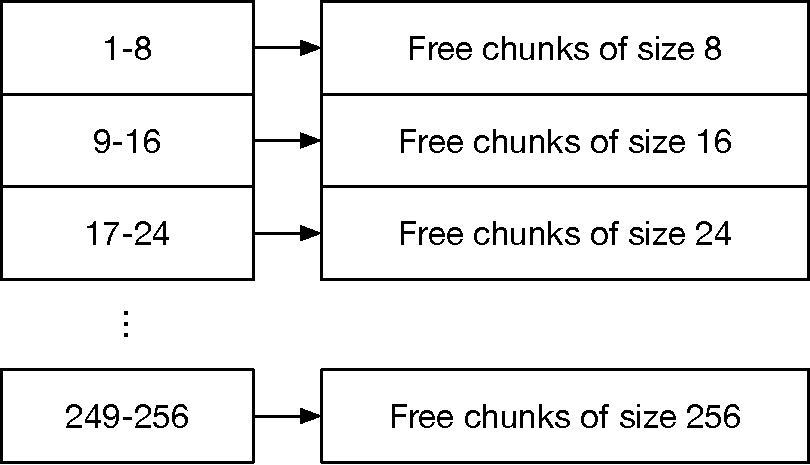
\includegraphics[width=10 cm]{fig1.free-lists.pdf}
  \caption{A visualization of the free lists in Python.}
  \label{fig:fig1}
\end{figure}

Internally, Python does this:

\begin{verbatim}
if (size <= 256) {
  // use small objs
} else {
  // use malloc
}
\end{verbatim}

Python's data types are very big and space-inefficient. For example, an integer is 24 bytes. A one-character string is 50 bytes, in stark contrast to C which is 2 bytes. Empty dictionaries in Python take up 240 bytes.

\subsection{Mechanics}

The mechanism is a linked list implementation of stacks. Using a request for a 48-byte object as an example:

\begin{enumerate}
	\setlength{\itemsep}{0pt}
	\setlength{\parskip}{3pt}
	\item The allocator goes to the 6th free list (48 bytes).
	\item If the free list is empty, it gets a chunk of memory from malloc and carves it into 48-byte chunks.
	\item An object is popped from the list.
	\item When free is called, that object is pushed back to the free list.
\end{enumerate}

Size classes are segregated in Python. If a 48-byte object is freed and is put back on the free list, it cannot be reused for requests for other sized-objects.

A problem can occur in the following situation:

\begin{enumerate}
	\setlength{\itemsep}{0pt}
	\setlength{\parskip}{3pt}
	\item 1 MB of 8-byte objects are allocated.
	\item All of them are freed.
	\item They all go back to the 8-byte free list. 1 MB of free memory is around.
	\item 1 MB of 16-byte objects are allocated.
	\item All of them are freed.
	\item The same goes on until there have been, say, 32 of such requests.
\end{enumerate}

In this case, actual memory usage will keep increasing but no memory is in use. Although the peak memory usage is 1 MB, the actual memory consumption is actually 32 MB---a 32x increase in memory!

\subsection{Notes on Python Lists}

Lists are implemented internally as vectors. Lists grow by doubling the size if the list is full and no longer fits new items. This is an instance of the \textit{ski rental problem}.

\subsubsection{Ski Rental Problem}

The ski rental problem is a problem where a decision to buy or a decision to rent is to be made. Using an example where renting a ski costs \$50, and buying a ski costs \$500. Assuming the skier rents in the beginning. At which point should the skier buy instead of renting?

Figure \ref{fig:fig2} shows the cumulative cost of renting ski and buying a ski over the number of times the skier skis. If the skier buys a ski at the point where the cost of renting skis and buying a ski meets (i.e. renting 10 times), the skier will never have to “lose” money as compared to continuing to rent after the point. The skier will not have to pay more than twice the amount of buying a ski.

\begin{figure}[ht!] %
\centering
	\begin{tikzpicture}
	\begin{axis}[axis lines = left, xlabel = Number of Skiing Activities, ylabel = Cost, ymin=0]
	\addplot[color=red, domain=0:20]{50*x};
	\addlegendentry{Renting}
	\addplot[color=blue, domain=0:20]{500};
	\addlegendentry{Buying}
	\end{axis}
	\end{tikzpicture}
	\caption{The cost of renting skiis versus buying a ski over the number of skiing activities.}
  	\label{fig:fig2}
\end{figure}

This strategy amortizes the cost of doubling, and is the optimal strategy in an environment with no information.

\section{Garbage Collection}

The most common garbage collection algorithm is mark-and-sweep. Reference counting is a common technique where the reference to a memory location is marked, and it cannot be removed until the count is zero. However this technique is incomplete, as the cases where we have self-referential pointers. So, there might still be certain sections of the memory which remain unclaimed after the garbage collection.

\begin{itemize}
	\itemsep 0cm
	\item Python, LISP, Java, PHP, JavaScript are some of the modern day computer languages which are garbage collected.
	\item Python’s GC is a reference counting GC, however a real better GC can be imported into it, using the \verb#gc# module.
\end{itemize}

\subsection{Mark-and-Sweep Algorithm}

Initially, all objects have a color bit set to white. All objects found by the collector are marked black. The remaining white objects are then considered unreachable and thus suitable for collection.

Essentially, this builds a transitive closure of the graph from the roots.

\subsection{Generational Garbage Collection}

This is a technique introduced by David Ungar, where objects are split into sections/classes/generations. It is mainly based on the concept that "most objects die young," so it makes sense to keep the immortal or objects which are not likely to die in a separate section, and not iterate through them while doing garbage collection, thus saving time.

\begin{itemize}
	\itemsep 0cm
	\item David Ungar and his team are mostly credited for making the Smalltalk language which was a super-dynamic language where everything is an object. It was a bad idea as it was super expensive. A JIT compilation was introduced as a workaround fix.
	\item His students associated with the group are the same team who later went on to build the V8 engine for the Google chrome browser.
	\item Generational GC takes pressure of the full heap GC. It can work quite well if can weak if lifetime is not much. Python uses approximate generational GC.
	\item In a generational GC, young objects or objects which are likely to be destroyed soon, are placed in a separate zone, and we apply our GC only on this set. This process is repeated over time. 
\end{itemize}

\end{document}
